\chapter{Shapley Explainability}

This chapter
is based on 
Refs.\cite{maz-shap-titanic}
and \cite{maz-shap-income},
which are highly recommended.


\label{ch-shapley}
``AI" is an ill-defined term. 
So is the term ``explainability". 
So the term ``Explainable 
AI (XAI)" is doubly ill-defined.
In 2018, the European Union codified 
an individual’s ``right to explanation" 
into a law called the General Data Protection 
Right (GDPR). This EU law was a strong 
motivation for Neural Net  
and boosted decision tree practitioners 
to come up with a way to enhance  
their machine learning algorithms
so that these comply with that law. Shapley 
explainability (SX) is 
one of the most popular 
methods for doing XAI.

So what does SX do? It ranks, for each individual 
of a population, the features (for example, race)
of a dataset, in the order of how influential those
features were in arriving at the decision the 
classifier made for that individual.

In my opinion, the goal of XAI is 
accomplished better with
bnets
 than with SX enhanced NNs.
SX ``explains", a posteriori, the outcome of a model, 
whereas bnets reveal the a priori process whereby 
that outcome was reached. Thus, SX can tell you 
that a model is racist, but it can't suggest 
how to fix it. On the other hand, if a bnet 
is acting racist, you don't have to throw it away. 
It can be fixed. 
Another
weakness of SX is that
it is quite expensive
computationally.
Bnets have explainability
built into them.
For bnets, explainability is
not an additional, and quite
onerous, calculation.
That is why I like to call 
bnets the gold standard of XAI.

Let

$F$ be the feature set. For example,
$F=\{age, gender, job\}$. 

$\calp(A)=
\{S: S\subset A \}$ be the power 
set of the set $A$ (i.e., the
set of all subsets of $A$, including
the empty set $\emptyset$).

$|\calp(A)|=\sum_{k=0}^{|A|} {|A|\choose k} =
\sum_{k=0}^{|A|} {|A|\choose k}1^k 1^{|A|-k}
= (1+1)^{|A|}=2^{|A|}$


$\calp_f(F)=\{S\in \calp(F): f\in S\}$
for $f\in F$, be all sets in $\calp(F)$
containing feature $f$. Note $\calp_f(F)= \calp(F)-\calp(F-\{f\})$

$\calp_{!f}(F)=\{S\in \calp(F): f\not\in S\}$
for $f\in F$, be all sets in $\calp(F)$
not containing feature $f$.
Note $\calp_{!f}(F)= \calp(F-\{f\})$



\begin{figure}[h!]
$$
\xymatrix{
&\emptyset\ar[dl]\ar[d]\ar[dr]
\\
\{age\}\ar[d]\ar[dr]
&\{gender\}\ar[dl]\ar[dr]
&\{job\}\ar[d]\ar[dl]
\\
\{age, gender\}\ar[dr]
&\{age, job\}\ar[d]
&\{gender,job\}\ar[dl]
\\
&\{{age}, gender, job\}
}$$
\caption{Graph of $\calp(F)$
for $F=\{age, gender, job\}$.
An arrow $H\larrow T$, where 
$H\in \calp(F)$ is the head of the arrow
and 
$T\in \calp(F)$ is the tail of the arrow,
means $H\supset T$
and $|H|=|T|+1$.}
\label{fig-pow-set-graph}
\end{figure}

Fig.\ref{fig-pow-set-graph}
shows a graph
of $\calp(F)$ for
$F=\{age, gender, job\}$.


Consider any $S\in \calp(F)$. Let

$N_{arr/nd}(S)= |S|=$ 
number of arrows entering
node $S$.

$N_{nds}(|S|)={|F|\choose |S|}=$ number
of nodes in level $|S|$ (i.e., row $|S|$). 

$N_{arr}(S)=N_{arr/nd}(S)
N_{nds}(|S|=|S|{|F|\choose |S|}=$
number of arrows 
going from row $|S|-1$ to row $|S|$.

\beq
P(S)=\frac{1}{N_{arr}(S)}
=\frac{1}{|S|
{|F|\choose |S|}}=
\frac{1}{|F|
{|F|-1\choose |S|-1}}
\;.
\eeq

\begin{claim}
\beq
\sum_{S\in \calp_{f}(F)} P(S)=1
\eeq
\end{claim}
\proof

\beqa
\sum_{S\in \calp_{f}(F)} P(S)&=&
\sum_{S\in \calp_{f}(F)}
\frac{1}{|F|
{|F|-1\choose |S|-1}}
\\
&=&
\sum_{k=1}^{|F|}
\sum_{S\in \calp_{f}(F)}
\indi(|S|=k)
\frac{1}{|F|
{|F|-1\choose k-1}}
\\
&=&
\sum_{k=1}^{|F|}
\frac{1}{|F|
{|F|-1\choose k-1}}
\underbrace{
\sum_{S\in \calp_{f}(F)}
\indi(|S|=k)}_{{|F|-1\choose k-1}}
\\&=& 1
\eeqa
\qed

Consider any $S\in\calp(F)$.
Henceforth, we will represent a
Machine Learning (ML) model
$ML_S$
as follows. 
$ML_S$  can be a Linear Regression ($LR_S$)
model, a Neural Net model ($NN_S$),
or any other type of ML model.
We will list a dataset; i.e., a 
set of tuples indexed by
the individuals $\s$
of a population $\Sigma$
such that $|\Sigma|=nsam$.
The independent variables 
of $ML_S$ (i.e., $x^\s_S=[x^\s_f : f\in S]$)
will be shown unboxed and the
 dependent variable 
(aka target feature) 
 (i.e., $y^\s$)
will be shown inside a box.
Then we will show an arrow with the
superscript ``ML-fit",
followed by the fit function
obtained by performing $ML_S$.


\beq
ML_S: \;\;\;\{(\s, x^\s_S,\boxed{y^\s}):\s\in 
\Sigma\}\mlarr \haty(x_S)
\eeq


For any feature $f\in F$
and individual $\s\in\Sigma$, 
define the {\bf Shapley Value} (SHAP) by

\begin{mdframed}[hidealllines=true,backgroundcolor=gray!10]
\beqa
SHAP^\s_f&=&
\sum_{S\in \calp_{f}(F)}
P(S)
\left[
\haty(x^\s_{S})-
\haty(x^\s_{S-\{f\}})
\right]
\\
&=&
E_S[\haty(x^\s_{S})-
\haty(x^\s_{S-\{f\}})
]
\eeqa
\end{mdframed}
Hence,
\begin{itemize}
\item
$SHAP^\s_f$ is an average over 
$\{ML_S: S\in \calp_f(F)\}$
for each individual $\s\in\Sigma$.
\item
$SHAP^\s_f$ averages 
the change in output $\haty$
when we change the model
from one without 
feature $f$ to one 
with feature $f$.
\item
$SHAP^\s_f$ can be 
negative or positive. Zero $SHAP^\s_f$
for individual $\s$
means feature $f$ does not influence 
how the decision $\haty$
was arrived at for individual $\s$.
\end{itemize}

\subsection{Numerical
examples of SHAP}
Next we present 2
numerical examples of SHAP.
The figures and numerical values
in this section
were taken directly
from 
Refs. \cite{maz-shap-titanic}
and \cite{maz-shap-income}.

\begin{enumerate}
\item {\bf Predicting Income from
$F=\{age, gender, job\}$.}

\begin{figure}[h!]
$$
\xymatrix{
&{\begin{array}{c}
S=\emptyset\\P(S)=0\\
\haty(x^\s_S)=\$50K
\end{array}}
\ar[dl]\ar[d]\ar[dr]
&& |S|=0
\\
\setprob{{\color{red}age}}{1/3}{40}
\ar[d]\ar[dr]
&\setprob{gender}{1/3}{48}
\ar[dl]\ar[dr]
&\setprob{job}{1/3}{100}
\ar[d]\ar[dl]
&|S|=1
\\
\setprob{{\color{red}age}, gender}{1/6}{39}
\ar[dr]
&\setprob{{\color{red}age}, job}{1/6}{85}
\ar[d]
&\setprob{gender,job}{1/6}{95}
\ar[dl]
&|S|=2
\\
&\setprob{{\color{red}age}, gender, job}{1/3}{83}
&& |S|=3
}$$
\caption{Same as Fig.\ref{fig-pow-set-graph},
but with added information
for a specific individual $\s$.
This figure 
contains enough information
to evaluate $SHAP^\s_{age}$.}
\label{fig-pow-set-graph-plus}
\end{figure}


Consider the problem of
predicting the
income of a person
based on the feature set
$F=\{age, gender, job\}$.
Suppose 
we are given a dataset
for this problem.   
We can train models
$ML_S$ for each $S\in \calp_{age}(F)$
where
$\haty$ is the income.
Then we can
calculate the matrix
$SHAP^\s_{age}$.
Fig.\ref{fig-pow-set-graph-plus}
gives all the information
necessary
to calculate $SHAP^\s_{age}$
for a single 
individual $\s$.


\beq
P(S)=\frac{1}{3{2\choose |S|-1}}=
\left\{
\begin{array}{ll}
\frac{1}{3{2\choose 0}}
=\frac{1}{3}
&\text{if $|S|=1$}
\\
\frac{1}{3{2\choose 1}}=\frac{1}{6}
&\text{if $|S|=2$}
\\
\frac{1}{3{2\choose 2}}=\frac{1}{3}
&\text{if $|S|=3$}
\end{array}\right.
\eeq

\beqa
SHAP^\s_{age}
&=&
\underbrace{P(age)}_{1/3}
\underbrace{[\haty(x^\s_{age})
-\haty(x^\s_\emptyset)]
}_{40K-50K}
\\
&+&
\underbrace{P(age,job)}_{1/6}
\underbrace{[\haty(x^\s_{age,job})
-\haty(x^\s_{job})]
}_{85K-100K}
\\
&+&
\underbrace{P(age,gender)}_{1/6}
\underbrace{[\haty(x^\s_{age,gender})
-\haty(x^\s_{gender})]
}_{39K-48K}
\\
&+&
\underbrace{P(age,gender,job)}_{1/3}
\underbrace{[\haty(x^\s_{age,gender,job})
-\haty(x^\s_{gender,job})]
}_{83K-95K}
\\
&=&-\$11.33K
\eeqa

\item {\bf Predicting passenger survival 
in the Titanic disaster.}





\begin{figure}[h!]
\centering
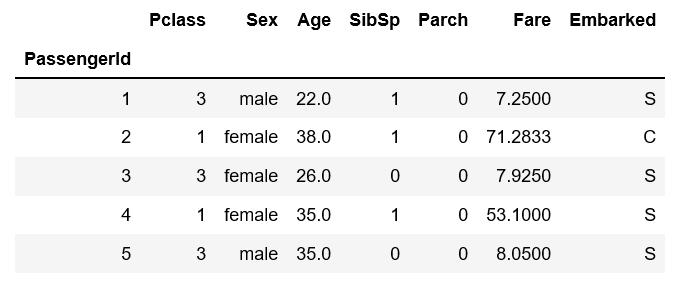
\includegraphics[width=4in]
{shapley/titanic-dataset-5.png}
\caption{
First five rows (passengers)
of an abridged version of the
Titanic Dataset
available at kaggle.com. 
This figure shows
$(\s, x^\s_F)$ for $\s=1,2,\ldots,5$.
It doesn't show the column $y^\s\in
\{died, survived\}$.
} 
\label{fig-titanic-dataset-5}
\end{figure}

\begin{figure}[h!]
\centering
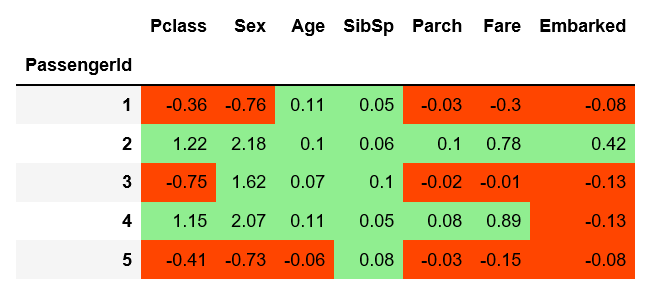
\includegraphics[width=4in]
{shapley/titanic-shap-table.png}
\caption{For Titanic dataset, a
table of $SHAP^\s_f$, where 
$\s\in \{1,2, \ldots 5\}$
and $f\in F$.
Cells with positive
SHAP are colored green,
and those with negative
SHAP are colored red.
The colors are not an
indication of whether
the passenger died or 
survived.
Note that the table
of a dataset and of $SHAP_f^\s$
have the same shape $(|\Sigma|, |F|)$.} 
\label{fig-titanic-shap-table}
\end{figure}

\begin{figure}[h!]
\centering
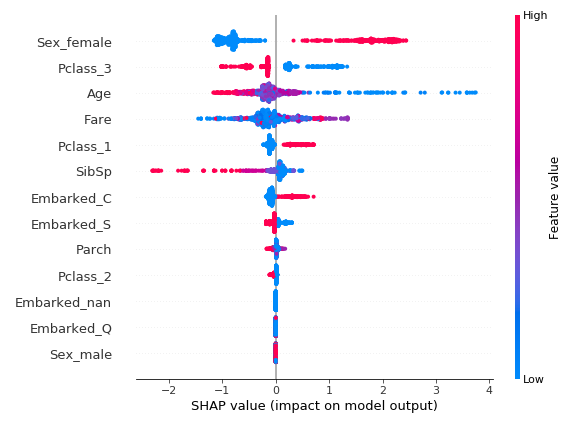
\includegraphics[width=4in]
{shapley/titanic-shap-plot.png}
\caption{For Titanic Dataset, a so called
``beeswarm" plot of $SHAP^\s_f$, where 
$\s\in \{1,2, \ldots, 891\}$
and $f\in F$.
In a beeswarm
plot, the thickness
of each row
is proportional to
how many 
individuals of the population
have that value 
of the $x$ coordinate.
This plot comes from 
Ref.\cite{maz-shap-titanic},
where it was generated using
the Titanic Dataset from kaggle.com and
the wonderful Python library ``SHAP".
The SHAP library can plot
Shapley Values 
in many other styles
besides this one.} 
\label{fig-titanic-shap-plot}
\end{figure}
\end{enumerate}

Consider the problem of
predicting 
whether an individual
will survive or not
based on a Titanic Dataset.
We can train models
$ML_S$ for each $S\in \calp(F)$
where
$\haty\in\{died, survived\}$.
Then we can
calculate the matrix
$SHAP^\s_f$
for all
individuals
$\s$
and features $f$.
Fig.\ref{fig-titanic-dataset-5}
shows the first 5
rows
of the Titanic Dataset.
Fig.\ref{fig-titanic-shap-table}
displays
$SHAP^\s_f$ in tabular
form and Fig.\ref{fig-titanic-shap-plot}
display $SHAP^\s_f$
in graphical form (as a beeswarm plot).